\documentclass{article}

\usepackage[letterpaper,top=3cm,bottom=2cm,left=3cm,right=3cm,marginparwidth=1.75cm]{geometry}

\usepackage{amsmath}
\usepackage{amssymb}
\usepackage{graphicx}
\usepackage{float}
\usepackage{algpseudocode}
\usepackage{multicol}
\usepackage[hidelinks]{hyperref}
\usepackage{xcolor}

\newcommand{\bigCI}{\mathrel{\text{\scalebox{1.07}{$\perp\mkern-10mu\perp$}}}}

\title{CPSC 322 Introduction to AI}
\author{Kaitian Xie}
\date{May 11, 2019}

\graphicspath{ {./images/} }

\begin{document}

\maketitle
\pagebreak

\tableofcontents
\pagebreak

\section{Introduction}

\subsection{What is AI?}

\begin{itemize}
    \item \textbf{Rationality}: an abstract ideal of intelligence, rather than ``whatever humans think/do''
    \item \textbf{Intelligent agents}: artifacts that act rationally in their environment:
        \begin{itemize}
            \item Actions are appropriate for their goals and circumstances.
            \item Flexible to changing environments and goals.
            \item Learn from experience.
            \item Make appropriate choices given perceptual limitations and limited resources.
        \end{itemize}
\end{itemize}

\subsection{Representation and Reasoning (R\&R) System}

\begin{itemize}
    \item A representational language to describe the environment and problems to be solved.
    \item Computational reasoning procedures to compute a solution to a problem.
\end{itemize}

\subsection{Representational Dimensions}

\begin{itemize}
    \item Problem types:
        \begin{itemize}
            \item \textbf{Static}: finding a solution doesn't involve reasoning into the future.
                \begin{itemize}
                    \item \textbf{Constraint satisfaction}: finding the state that satisfies set of constraints.
                    \item \textbf{Answering query}: is a given proposition true/likely given what is known?
                \end{itemize}
            \item \textbf{Sequential}: finding a solution requires looking for a number of steps into the future.
                \begin{itemize}
                    \item \textbf{Planning}: finding the sequence of actions to reach a goal state/maximize.
                \end{itemize}
        \end{itemize}
\end{itemize}

\subsection{Deterministic vs. Stochastic}

\begin{itemize}
    \item \textbf{Sensing uncertainty}: the agent cannot fully observe the current state of the world.
    \item \textbf{Effect uncertainty}: the agent doesn't know for sure the effects of its actions.
\end{itemize}

\subsection{States, Features, and Relationships}

\begin{itemize}
    \item An environment can be modelled in terms of states, features, and relationships.
\end{itemize}

\section{Search}

\subsection{Intro to Search}

\subsubsection{Directed Acyclic Graph (DAG)}

\begin{itemize}
    \item \textbf{Directed ayclic graph}: a graph with no cycles and where the arcs have associated directions.
\end{itemize}

\subsubsection{Search with Costs}

\begin{itemize}
    \item \textbf{Cost of a path}: sum of costs of its arcs $cost(<n_0, \ldots, n_k>) = \sum\limits_{i=1}^{k} (<n_{i-1}, n_i>)$
    \item \textbf{Optimal solution}: solution with minimal cost.
\end{itemize}

\subsubsection{Heuristic}

\begin{itemize}
    \item \textbf{Search heuristic ($h(n)$)}: an estimate of the cost of the lowest-cost path from node $n$ to a goal node.
    \item \textbf{Admissible heuristic}: $h(n)$ is admissible if it is never an overestimate, i.e. $h(n)$ is a lower bound. To construct an admissible heuristic, we can either:
    \begin{itemize}
        \item drop some constraints or
        \item make less restrictions on actions
    \end{itemize}
    \item \textbf{Dominance}: If $h_2(n) \geq h_1(n)$ for every state $n$ (both admissible), then $h_2$ dominates $h_1$.
    \item we can combine two admissible heuristic functions: $h(n) = max\{h_1(n), h_2(n)\}$.
\end{itemize}

\subsubsection{Uninformed Search vs Heuristic Search}

\begin{itemize}
    \item \textbf{Uninformed}: not taking the goal into account until the goal state is reached.
    \item \textbf{Heuristic}: there exists extra knowledge to guide the search.
\end{itemize}

\subsection{Generic Search Algorithm}

\begin{algorithmic}
    \Require{a graph, a start node $n_0$, $goal(n)$}
    \State{$frontier := [<n_0>]$}
    \While{$frontier$ is not empty}
        \State{Select and remove a path $<n_0, \ldots, n_k>$ from $frontier$}
        \If{$goal(n_k)$}
            \State{return $<n_0, \ldots, n_k>$}
        \EndIf
        \For{every neighbor $n$ of $n_k$}
            \State{Add $<n_0, \ldots, n_k, n>$ to $frontier$}
        \EndFor
    \EndWhile
\end{algorithmic}

\begin{itemize}
    \item How paths are selected from the $frontier$ defines the search strategy.
    \item The order in which paths are added to $frontier$ is not specified.
\end{itemize}

\begin{figure}[H]
    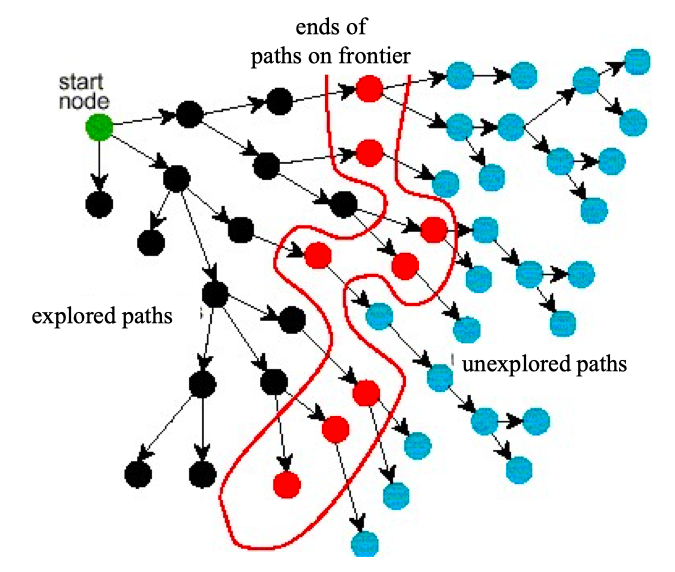
\includegraphics[width=\textwidth]{generic_search_algo_visualization}
    \centering
\end{figure}

\subsubsection{Branching Factor (b)}

\begin{itemize}
    \item \textbf{Forward branching factor}: number of arcs going out of a node
    \item \textbf{Backward branching factor}: number of arcs going into a node
\end{itemize}

\subsubsection{Complete \& Optimal}

\begin{itemize}
    \item \textbf{Complete}: can find a solution.
    \item \textbf{Optimal}: can find the best solution.
\end{itemize}

\subsubsection{Complexity}

\begin{itemize}
    \item \textbf{Time complexity}: amount of time needed in the worst-case scenario; expressed in terms of maximum path length ($m$) and maximum branching factor ($b$).
    \item \textbf{Space complexity}: amount of space needed in the worst-case scenario; expressed in terms of $m$ \& $b$.
\end{itemize}

\subsection{Depth-First Search (DFS)}

\begin{itemize}
    \item $frontier$ is a stack $[p_1, p_2, \ldots, p_k]$
    \item neighbors of last node of $p_1$ are $\{n_1, \ldots, n_k\}$
    \item
    \begin{algorithmic}
        \While{$frontier$ is not empty}
            \State{$p := frontier.pop()$}
            \State{$n_{end} := $ last node of $p$}
            \If{$goal(n_{end})$}
                \State{Return $p$}
            \EndIf
            \State{$frontier.push((p, n_1), \ldots, (p, n_k))$}
        \EndWhile
    \end{algorithmic}
    \item not complete because DFS may get ``stuck'' in a graph that has cycles.
    \item not optimal because DFS may return a longer solution while a shorter solution exists
    \item time complexity: $O(b^m)$
    \item space complexity: $O(bm)$
    \item DFS is appropriate when:
        \begin{itemize}
            \item space is restricted.
            \item there are many solutions, perhaps with long path solutions, particularly for the case in which all paths lead to a solution.
        \end{itemize}
    \item DFS is inappropriate when:
        \begin{itemize}
            \item cycles
            \item shallow solution
            \item optimality is needed
        \end{itemize}
\end{itemize}

\subsection{Breadth-First Search}

\begin{itemize}
    \item $frontier$ is a queue $[p_1, p_2, \ldots, p_k]$
    \item neighbors of last node of $p_1$ are $\{n_1, \ldots, n_k\}$.
    \item
    \begin{algorithmic}
        \While{$frontier$ is not empty}
            \State{$p := frontier.poll()$}
            \State{$n_{end} := $ last node of $p$}
            \If{$goal(n_{end})$}
                \State{Return $p$}
            \EndIf
            \State{$frontier.offer((p, n_1), \ldots, (p, n_k))$}
        \EndWhile
    \end{algorithmic}
    \item complete because it doesn't get stuck in cycles
    \item optimal because it guarantees to find the path that involves the fewest paths
    \item time complexity: $O(b^m)$
    \item space complexity: $O(b^m)$
\end{itemize}

\subsection{Iterative Deepening Search}

\begin{itemize}
    \item
        \begin{itemize}
            \item Look with DFS for solution at depths $1, 2, \ldots$
            \item If a solution can't be found at depth $D$, try again at depth $D+1$
            \item depth-bounded depth-first searcher
            \item given a bound $B$, assume the paths of length $B$ can't be expanded.
        \end{itemize}
    \item time complexity: $O(b^m)$

    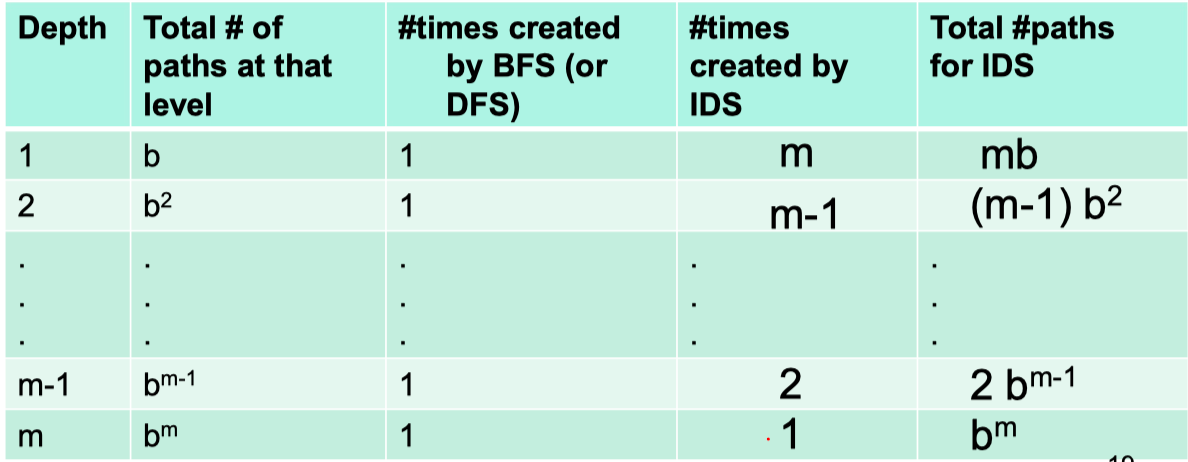
\includegraphics[scale=0.3]{ids_time_complexity}
    
    \begin{align*}
        b^m  + 2b^{m-1} + 3b^{m-2} + \ldots + mb 
        &= b^m (1 + 2b^{-1} + 3b^{-2} + \ldots + mb^{1-m}) \\
        & \leq b^m \sum\limits_{i=1}^{\infty} ib^{1-i} \\
        &= b^m (\frac{b}{b-1})^2 \\
        &= O(b^m)
    \end{align*}
    \item space complexity: $O(mb)$
\end{itemize}

\subsection{Lowest-Cost-First Search (LCFS)}

\begin{itemize}
    \item
    \begin{itemize}
        \item Select a path with the lowest cost from $frontier$ (a priority queue).
        \item not complete if there exists a cycle with zero or negative arc costs, otherwise it is complete
        \item not optimal if negative costs exist, otherwise it is optimal
        \item time complexity: $O(b^m)$
        \item space complexity: $O(b^m)$
            \begin{itemize}
                \item if costs are equal $\Rightarrow$ BFS
            \end{itemize}
    \end{itemize}
\end{itemize}

\subsection{Best-First Search}

\begin{itemize}
    \item Select a path from the $frontier$ with minimal h-value (for the end node).
    \item The $frontier$ is implemented by a priority queue order by h-value.
    \item This is a greedy approach since it always takes a locally best path.
    \item not complete: if there exist low h-values in a cycle, BestFS gets stuck.
    \item not optimal: a heuristic might be misleading.
    \item time complexity: $O(b^m)$
    \item space complexity: $O(b^m)$
    \item BestFS is appropriate when:
        \begin{itemize}
            \item $h(n)$ is very good.
        \end{itemize}
\end{itemize}

\subsection{A*}

\begin{itemize}
    \item LCFS + BestFS
    \item $f(p) = cost(p) + h(p)$
    \item The $frontier$ is implemented by a priority queue ordered by f-value.
    \item $A^{*}$ always selects a path that has the lowest estimated total distance to a goal.
    \item complete: $A^{*}$ always tests shorter underestimate of the total cost, so not missing anything
    \item optimal: $A^{*}$ is optimal if:
        \begin{itemize}
            \item $b$ is finite
            \item costs are strictly positive
            \item $h(n)$ is non-negative and admissible
        \end{itemize}
    \item proof of optimality: \textit{Lecture 8 slides 24-32}
    \item optimal efficiency: among all optimal algorithms that start from the same start node and use the same heuristic, $A^{*}$ expands the minimal number of paths.
    \item time complexity: $O(b^m)$
    \item space complexity: $O(b^m)$
\end{itemize}

\subsection{Branch-and-Bound Search (B\&B)}

\begin{itemize}
    \item $frontier$ implemented a stack, similar to DFS
    \item order of adding neighbours can be customized
    \item keeps track of a lower bound and an upper bound on a each path:
        \begin{itemize}
            \item lower bound: $LB(p) = f(p) = cost(p) + h(p)$
            \item upper bound: $UB = \text{cost of the best solution found so far}$ (initialize $UB = \infty$)
        \end{itemize}
    \item when a path $p$ is selected for expansion
        \begin{itemize}
            \item if $LB \geq UB$: remove $p$ from $frontier$
            \item else expand $p$
        \end{itemize}
    \item not complete: B\&B gets stuck in a graph with cycles
    \item optimal, but not optimal efficient
    \item time complexity: $O(b^m)$
    \item space complexity: $O(mb)$ (like DFS)
\end{itemize}

\subsection{Iterative Deepening A* (IDA*)}

\begin{itemize}
    \item search depth-first, but to a fixed depth/bound
    \item depth measured in f-values
    \item if you don't find a solution, update the bound with the lowest f-value that passed the previous bound
    \item time complexity: $O(b^m)$
    \item space complexity: $O(mb)$
\end{itemize}

\subsection{Memory-Bounded A* (MBA*)}

\begin{itemize}
    \item keep $frontier$ in memory as we can
    \item if we need to free some memory, we delete:
        \begin{itemize}
            \item the worst paths (with highest f-values)
            \item ``back them up'' to a common ancestor
            \item update $h(n)$ of the ancestor if possible
        \end{itemize}
\end{itemize}

\subsection{Summary of Search Strategies}

\begin{figure}[H]
    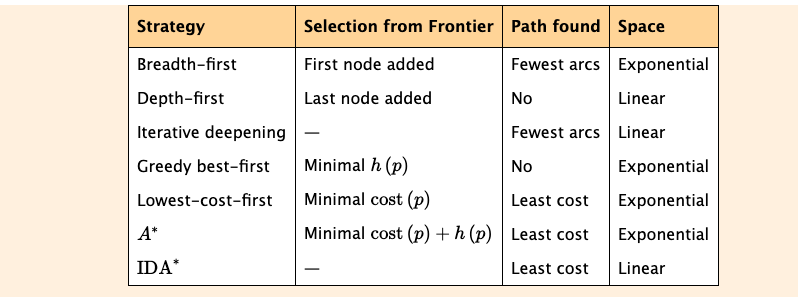
\includegraphics[width=\textwidth]{summary_of_search_strategies}
    \centering
\end{figure}

\subsection{Cycle Checking}

\begin{itemize}
    \item Prune a path that ends in a node already on the path
    \item Pruning doesn't remove an optimal solution.
    \item linear time complexity
\end{itemize}

\subsection{Multiple-Path Pruning}

\begin{itemize}
    \item Prune a path to node $n$ that you already found a path to.
\end{itemize}

\section{CSP}

\subsection{Variables/Features, Domains, and Possible Worlds}

\begin{itemize}
    \item Capital letters to represent variables.
    \item \textbf{Domain}: $dom(V)$ = possible values for $V$.
    \item \textbf{Possible world}: a complete assignment of values to a set of variables.
\end{itemize}

\subsection{Constraints}

\begin{itemize}
    \item \textbf{Constraint}: restrictions on the values for one or more variables.
        \begin{itemize}
            \item function that returns true when given values for each variable satisfy the constraint
            \item list of valid domain values for each variable participating in the constraint
        \end{itemize}
    \item \textbf{Unary constraint}: restriction involving a single variable.
    \item \textbf{K-ary constraint}: restriction involving the domains of $k$ different variables.
        \begin{itemize}
            \item can be represented as unary constraints.
        \end{itemize}
\end{itemize}

\subsection{Constraint Satisfaction Problems (CSP)}

\begin{itemize}
    \item \textbf{Constraint satisfaction problem} consists of:
    \begin{itemize}
        \item a set of variables
        \item a domain for each variable
        \item a set of constraints
    \end{itemize}
    \item \textbf{Model} is an assignment of values to variables (i.e. possible world) that satisfies all of the constraints.
\end{itemize}

\subsection{Generate-and-Test Algorithm}

\begin{algorithmic}
    \For{$a$ in $domA$}
        \For{$b$ in $domB$}
            \For{$c$ in $domC$}
                \If{$abc$ satisfies all constraints}
                    \State \Return{$abc$}
                \EndIf
            \EndFor
        \EndFor
    \EndFor
    \State \Return {$NULL$}
\end{algorithmic}

\begin{itemize}
    \item can solve any CSP
    \item bad runtime
\end{itemize}

\subsection{CSPs as Search Problems}

\begin{itemize}
    \item \textbf{States}: assignments of values to a subset of the variables.
    \item \textbf{Start state}: the empty assignment.
    \item \textbf{Neighbours}: nodes in which values are assigned to one additional variable.
    \item \textbf{Goal(n)}: set of constraints
    \item \textbf{Goal state}: a state which assigns a value to each variable, and satisfies all of the constraints.
    \item \textbf{Solution}: possible world that satisfies the constraints.
    \item \textit{Note}: 
        \begin{itemize}
            \item Path is unimportant.
            \item depth = num of variables
            \item $h(n)$ is useless since all solutions have the same distance from the goal
            \item The tree is finite and has no cycles.
        \end{itemize}
    \item We use \underline{DFS} as our search strategy.
    \item Pruning: if an end node violates one or more constraints, we a solution cannot exist beyond that node $\Rightarrow$ remove that path.
    \item Efficiency depends on the order in which variables are expanded.
    \item \textbf{Degree ``heuristics''}: choosing variables invovled in more constraints is better.
\end{itemize}

\subsection{Consistency}

\begin{itemize}
    \item Prune domains before searching.
    \item \textbf{Domain consistency}: a variable is domain consistent if no value of its domain is ruled impossible by any unary constraint.
    \item \textbf{Constraint network}: a graph with
        \begin{itemize}
            \item one node for every variable
            \item one node for every constraint
            \item undirected edges between variable nodes and constraint nodes
        \end{itemize}
    \item \textbf{Arc consistency}: an arc $<x, r(x, y)>$ is consistent if for each value $x$ in $dom(X)$, there is some value $y$ in $dom(Y)$ such that $r(x, y)$ is satisfied. A network is arc consistent if all its arcs are consistent.
        \begin{itemize}
            \item To enforce arc consistency, we remove $x$ from $dom(X)$ is there is no value $dom(Y)$ to satisfy the constraint.
        \end{itemize}
\end{itemize}

\subsection{Arc Consistency Algorithm}

\begin{itemize}
    \item General idea:
        \begin{enumerate}
            \item Go through all the arcs.
            \item Make each arc consistent by pruning if needed.
            \item Reconsider consistent arcs that could be made inconsistent again by this pruning.
            \item Eventually reach a ``fixed point'': all arcs are consistent.
        \end{enumerate}
    \item Pseudo-code:
        \begin{algorithmic}
            \State{$TDA \gets \text{all arcs in Constraint Network}$}
            \While{$TDA$ is not empty}
                \State{Select an arc $a$ from $TDA$}
                \If{$a$ is not consistent}
                    \State{Make $a$ consistent}
                    \State{Add arcs to $TDA$ that may now be inconsistent}
                \EndIf
            \EndWhile
        \end{algorithmic}
    \item Detailed version:
        \begin{figure}[H]
            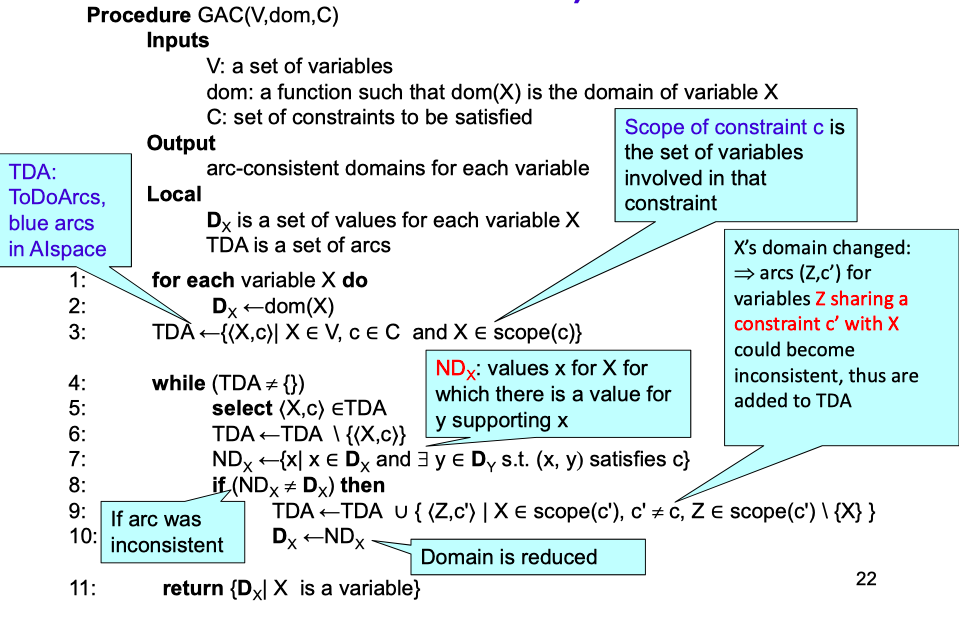
\includegraphics[width=\textwidth]{gac}
            \centering
        \end{figure}
    \item Complexity (Worst-case)
        \begin{itemize}
            \item $d = \text{max size of a variable domain}$
            \item $n = \text{number of variables}$
            \item Assume all constraints are binary.
            \item Max number of binary constraints = $\frac{n * (n - 1)}{2}$
            \item The same arc can be inserted in $TDA$ $d$ times.
            \item $d^2$ steps are involved in checking the consistency of an arc.
            \item Overall complexity: $O(n^2d^3)$, better than DFS.
        \end{itemize}
    \item Outcomes:
        \begin{enumerate}
            \item One domain is empty $\Rightarrow$ no solution.
            \item Each domain has a single value $\Rightarrow$ unique solution.
            \item Some domains have more than one value $\Rightarrow$ zero or more solutions.
                \begin{itemize}
                    \item Arc consistency is not good enough $\Rightarrow$ we still need to search.
                \end{itemize}
        \end{enumerate}
\end{itemize}

\subsection{Domain Splitting}

\begin{itemize}
    \item Split a problem in a number of disjoint cases, so $sol(CSP) = \bigcup\limits_{i} sol(CSP_i)$.
    \item By splitting, we may be able to run AC again. However, we need to keep all CSPs around.
    \item Arc consistency + domain splitting:
        \begin{itemize}
            \item \textbf{States}: $vector(D(V_1), \ldots, D(V_2))$ of remaining domains, with $D(V_i) \subseteq dom(V_i)$ for each $V_i$.
            \item \textbf{Start state}: vector of original domains $(dom(V_i), \ldots, dom(V_n))$
            \item \textbf{Successor function}: reduce one of the domains + run arc consistency
            \item \textbf{Goal state}: vector of unary domains that satisfy all constraints:
                \begin{itemize}
                    \item only one value left for each variable
                    \item assignment of each variable to its single value is a model
                \end{itemize}
            \item \textbf{Solution}: that assignment
        \end{itemize}
    \item \#CSPs to keep at a time: $O(bm)$
\end{itemize}

\subsection{Local Search}

\begin{itemize}
    \item general idea:
        \begin{enumerate}
            \item Start from a possible world.
            \item Generate some neighbors.
            \item Move from the current node to a neighbor.
        \end{enumerate}
    \item \textbf{CSP}: a set of variables, domains for these variables, and constraints on their joint values.
    \item \textbf{Node}: a complete assignment to all of the variables.
    \item \textbf{Neighbor relation}: specified by some small incremental change to the variable assignment.
    \item \textbf{Scoring function}: judges cost of a node (want to minimize).
    \item \textbf{Iterative best improvement}: selects the neighbor that optimizes some evaluation function (minimal number of constraint violations).
        \begin{itemize}
            \item \textbf{Evaluation function (h(n))}: number of constraint violations in state $n$.
            \item \textbf{Greedy descent}: evaluates $h(n)$ for each neighbor, picks the neighbor $n$ with minimal $h(n)$.
            \item \textbf{Hill climbing}: equivalent algorithm for maximization problems (maximizes the number of satisfied constraints).
        \end{itemize}
    \item
        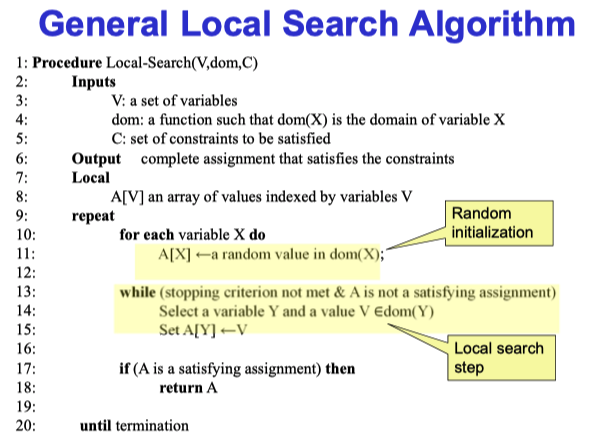
\includegraphics[scale=0.6]{general_local_search_algorithm}
    \item Only the current node is kept at each step $\Rightarrow$ no backtracking
    \item Most research in local search is about finding effective mechanisms for escaping from local minima. The iterative best improvement gets tapped in locally optimal minima.
\end{itemize}

\subsection{Stochastic Local Search (SLS)}

\begin{itemize}
    \item \textbf{Start node}: random assignment
    \item \textbf{Goal}: assignment with zero unsatisfied constraints
    \item \textbf{Heuristic function (h)}: \# unsatisfied constraints
    \begin{itemize}
        \item the lower, the better
    \end{itemize}
    \item SLS is a mix of 
    \begin{itemize}
        \item \textbf{Greedy descent}: move to a neighbor with lowest $h$
        \item \textbf{Random walk}: take some random steps, i.e. move to neighbor with some randomness
        \item \textbf{Random restart}: reassigning values to all variables
    \end{itemize}
\end{itemize}

\subsection{Greedy Descent vs Random Sampling}

\begin{itemize}
    \item \textbf{Greedy descent}:
        \begin{itemize}
            \item good for finding local minima
            \item bad for exploring new parts of the search space
        \end{itemize}
    \item \textbf{Random sampling}:
        \begin{itemize}
            \item good for exploring new parts of the search space
            \item bad for finding local minima
        \end{itemize}
\end{itemize}

\subsection{Selecting Neighbors}

\begin{itemize}
    \item \textbf{One stage selection}:
        \begin{itemize}
            \item the best neighbor
            \item a random variable-value pair
        \end{itemize}
    \item \textbf{Two stage selection} (first select variable $V$, then new value for $V$):
        \begin{itemize}
            \item selecting variables:
                \begin{itemize}
                    \item the variable which participates in the largest number of conflicts
                    \item a random variable that participates in some conflict
                    \item a random variable
                \end{itemize}
            \item selecting rules:
                \begin{itemize}
                    \item the best value for the chosen variable
                    \item a random value for the chosen variable
                \end{itemize}
        \end{itemize}
\end{itemize}

\subsection{Comparing SLS Algorithms}

\begin{itemize}
    \item Time taken is a random variable.
    \item Runtime variations of 2 order of magnitude in repeated runs.
    \item Stagnation $\Rightarrow$ $\infty$ mean runtime
    \item Runtime distribution
        \begin{itemize}
            \item x-axis: runtime/number of steps
            \item y-axis: proportion/number of runs solved in that runtime
            \item mean/median/mode runtime doesn't tell the whole story.
        \end{itemize}
\end{itemize}

\subsection{SLS Variants}

\begin{itemize}
    \item \textbf{Simulated annealing}
        \begin{itemize}
            \item Key idea: Change the degree of randomness.
            \item Annealing: a metallurgical process where metals are heated and then slowly cooled.
                \begin{itemize}
                    \item starts with high tendency to take random steps.
                    \item over time, more likely to follow the scoring function.
                \end{itemize}
            \item Algorithm:
                \begin{itemize}
                    \item At the node $n$. Pick a variable at random and a new value at random. Generate $n'$.
                    \item if $n'$ is an improvement ($h(n) - h(n') > 0$, adopt it; otherwise, adopt it with a probability: $e = \frac{h(n) - h(n')}{T}$
                \end{itemize}
            \item If $T$ decreases slow enough, then simulated annealing search will find a global optimum with probability approaching 1.
        \end{itemize}
    \item \textbf{Taboo Search}
        \begin{itemize}
            \item Make partial assignments as Taboo.
            \begin{itemize}
                \item stops repeatedly visiting the same (or similar) local minima.
            \end{itemize}
            \item A queue of $k$ variable-value pairs that are taboo.
                \begin{itemize}
                    \item $k$ needs to be optimized empirically.
                \end{itemize}
        \end{itemize}
    \item \textbf{Population Based SLS}
        \begin{itemize}
            \item Maintain a population of $k$ individuals
                \begin{itemize}
                    \item At every stage, update your population.
                    \item Whenever one individual is a solution, report it.
                \end{itemize}
        \end{itemize}
    \item \textbf{SLS for Constraint Optimization Problems}
        \begin{itemize}
            \item constraint optimization problems
                \begin{itemize}
                    \item hard constraints: need to satisfy all of them.
                    \item soft constraints: need to satisfy them as well as possible.
                    \item can have weighted constraints:
                        \begin{itemize}
                            \item minimize $h(n)$ = sum of weights of unsatisfied constraints in $n$.
                            \item hard constraints have large weights.
                            \item some soft constraints can be more important than other soft constraints $\Rightarrow$ larger weights.
                        \end{itemize}
                \end{itemize}
        \end{itemize}
\end{itemize}

\section{Planning}

\subsection{Intro to Planning}

\begin{itemize}
    \item \textbf{Planning}: build a sequence of actions that, if executed, takes the agent from the current state to a state that achieves a goal.
        \begin{itemize}
            \item Both states and actions as set of features.
            \item Actions as preconditions and effects defined on state features.
            \item Agent can reason more deliberately about which actions to consider to achieve its goals.
        \end{itemize}
    \item A planning problem can be solved as a pure search problem or CSP.
    \item Delivery Robot Example (Lecture 16 slides 13 - 16)
    \item STRIPS representation:
        \begin{itemize}
            \item An action has two parts:
                \begin{itemize}
                    \item \textbf{Preconditions}: a set of assignments to variables that must be satisfied in order for the action to be legal/valid/applicable.
                    \item \textbf{Effects}: a set of assignments to variables that are caused by the action.
                \end{itemize}
        \item \textbf{Assumption}: all features not explicitly changed by an action stay unchanged
        \item Example (Lecture 16 slides 20 - 22)
        \end{itemize}
\end{itemize}

\subsection{Forward Planning}

\begin{itemize}
    \item Search in the state-space graph:
        \begin{itemize}
            \item \textbf{States}: possible worlds (full assignments of values to features).
            \item \textbf{Arcs}: possible actions in state $s$.
            \item \textbf{Plan}: a path from the initial state to a state that satisfies the goal.
            \item \textbf{Solution}: a sequence of actions to reach the goal
        \end{itemize}
    \item Standard Search vs. Specific R\&R Systems
        \begin{multicols}{2}
            CSP
            \begin{itemize}
                \item \textbf{State}: assignments to a subset of the variables.
                \item \textbf{Successor function}: assign values to a ``free'' variable.
                \item \textbf{Goal test}: set of constraints.
                \item \textbf{Solution}: possible world that satisfies the constraints.
                \item \textbf{Heuristic funciton}: none (all solutions at the same distance from start)
            \end{itemize}
            
            \columnbreak
            
            Planning
            \begin{itemize}
                \item \textbf{State}: full assignments of values to features
                \item \textbf{Success function}: states reachable by applying actions with preconditions satisfied in the current state.
                \item \textbf{Goal test}: partial assignment of values to features.
                \item \textbf{Solution}: a sequence of actions.
                \item \textbf{Heuristic function} (see below)
            \end{itemize}
        \end{multicols}
        \item Heuristics for forward planning: number of actions needed to get from $s$ to goal.
            \begin{itemize}
                \item \textbf{Sub-goal}: a particular assignment for one of the features in the goal
                \item 2 simplifications:
                    \begin{itemize}
                        \item all features are binary: T/F
                        \item goals and preconditions can only be assignments to T
                    \end{itemize}
                \item Each action has add list and delete list:
                    \begin{itemize}
                        \item \textbf{Add list}: features made T by the action.
                        \item \textbf{Delete list}: features made F by the action
                    \end{itemize}
                \item Strategies:
                    \begin{itemize}
                        \item Ignore delete list.
                        \item Count number of unsatisfied sub-goals.
                        \item Ignore action preconditions.
                    \end{itemize}
            \end{itemize}
        \item Forward planning works well
            \begin{itemize}
                \item in combination with other techniques.
                \item for specific domains.
            \end{itemize}
\end{itemize}

\subsection{Planning as CSP}

\begin{itemize}
    \item Constraints:
        \begin{itemize}
            \item \textbf{Initial state constraints}: constrain the state variables at time 0, i.e. before any actions has occurred.
            \item \textbf{Goal constraints}: constrain at some time $k$, where $k$ is the horizon.
            \item \textbf{Precondition constraints}: constraints between state variables at time $t$ and actions at time $t$, i.e. they specify what must hold for an action to take place.
            \item \textbf{Effect constraints}: constraints between state variables at time $t$, actions at time $t$, and state variables at time $t + 1$, i.e. a state variable at time $t + 1$ is affected by actions at time $t$ and its own previous value at time $t$.
        \end{itemize}
    \item Variables: states and actions
    \item Constraints relate to states at a given time $t$, the corresponding valid actions and the resulting states at $t + 1$.
    \item \textbf{Horizon k}: ``unrolling the plan'' for a fixed number of steps.
        \begin{itemize}
            \item Construct a CSP variable for each STRIPS state variable at each time step from $0$ to $k$.
            \item Construct a boolean CSP variable for each STRIPS action at each time step from $0$ to $k - 1$.
        \end{itemize}
\end{itemize}

\section{Logic}

\subsection{Intro to Logic}

\begin{itemize}
    \item \textbf{Syntax}: specifies the symbols used, and how they can be combined to form legal sentences.
        \begin{itemize}
            \item \textbf{Knowledge base}: set of sentences in the language
        \end{itemize}
    \item \textbf{Semantics}: specifies the meaning of symbols and sentences.
    \item \textbf{Reasoning theory/proof procedure}: a specification of how an answer can be produced
        \begin{itemize}
            \item \textbf{Sound}: only generates correct answers with respect to the semantics
            \item \textbf{Complete}: guaranteed to find an answer if it exists.
        \end{itemize}
\end{itemize}

\subsection{Propositional Definite Clause Logic (PDCL)}

\begin{itemize}
    \item Syntax
        \begin{itemize}
            \item \textbf{Atom}: symbol starting with a lower case letter.
            \item \textbf{Body}: 
                \begin{itemize}
                    \item atom
                    \item of the form $b_1 \wedge b_2$ ($b_1$ and $b_2$ are bodies)
                \end{itemize}
            \item \textbf{Definite clause}:
                \begin{itemize}
                    \item atom
                    \item rule of the form $h \leftarrow b$ ($h$ is an atom and $b$ is a body)
                        \begin{itemize}
                            \item ``$h$ if $b$''
                        \end{itemize}
                \end{itemize}
            \item \textbf{Knowledge base (KB)}: set of definite clauses.
        \end{itemize}
    \item Semantics
        \begin{itemize}
            \item \textbf{Interpretation I} assigns a truth value to each atom.
            \item Use the interpretation to determine the truth values of clauses:
                \begin{itemize}
                    \item A body $b_1 \wedge b_2$ is true in I if and only if $b_1$ is true in I and $b_2$ is true in I.
                    \item A rule $h \leftarrow b$ is false in I if and only if $b$ is true in I and $h$ is false in I.
                    \item A KB is true in I if and only if every clause in KB is true in I.
                    \item A model of KB is an interpretation in which KB is true.
                \end{itemize}
            \item If $KB$ is a set of clauses and $G$ is a conjunction of atoms, G is a logical consequence of KB ( $KB \vDash G$) if $G$ is true in every model of $KB$.
        \end{itemize}
\end{itemize}

\subsection{Proof Procedures}

\begin{itemize}
    \item \textbf{Proof procedure}: a mechanically derivable demonstration that a formula logically follows from a KB.
    \item Given a proof procedure $P$, $KB \vdash_P g$ means $g$ can be derived from KB with the proof procedure.
    \item A proof procedure $P$ is sound if $KB \vdash_P g$ implies $KB \vDash g$.
    \item A proof procedure $P$ is complete if $KB \vDash g$ implies $KB \vdash_P g$.
\end{itemize}

\subsection{Bottom-Up Proof Procedure}

\begin{itemize}
    \item Proof procedure:
    \begin{algorithmic}
        \State{$C \gets \{\}$}
        \Repeat
            \State{Select clause $h \rightarrow b_1 \wedge \ldots \wedge b_m$ in $KB$ such that $b_i \in C$ for all $i$, and $h \notin C$}
            \State{$C \gets C \cup \{h\}$}
        \Until{no more clauses can be selected}
    \end{algorithmic}
    
    $KB \vdash G$ if $G \subseteq C$ at the end of this procedure ($C$ is a fixed point).
    \item 
    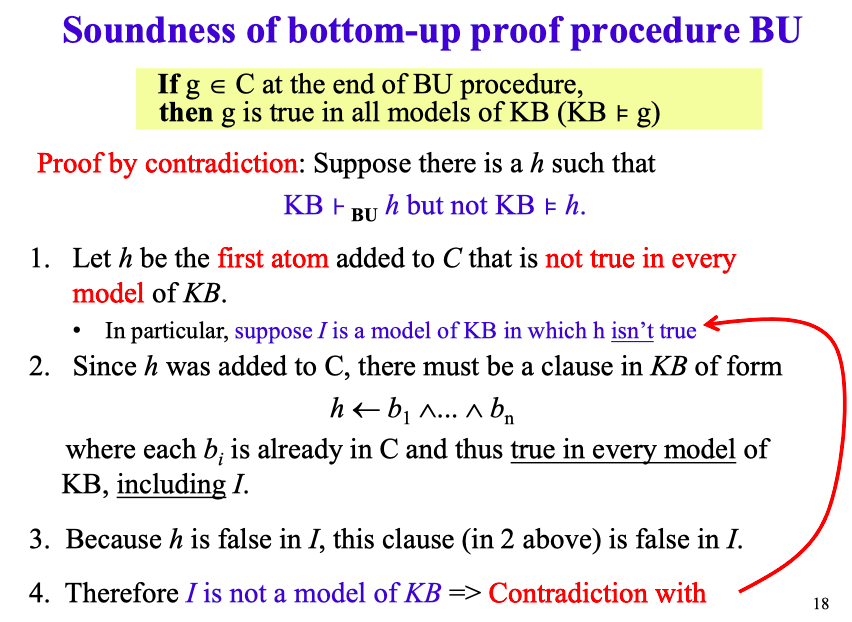
\includegraphics[scale=0.45]{soundness_of_bu}
    \item
    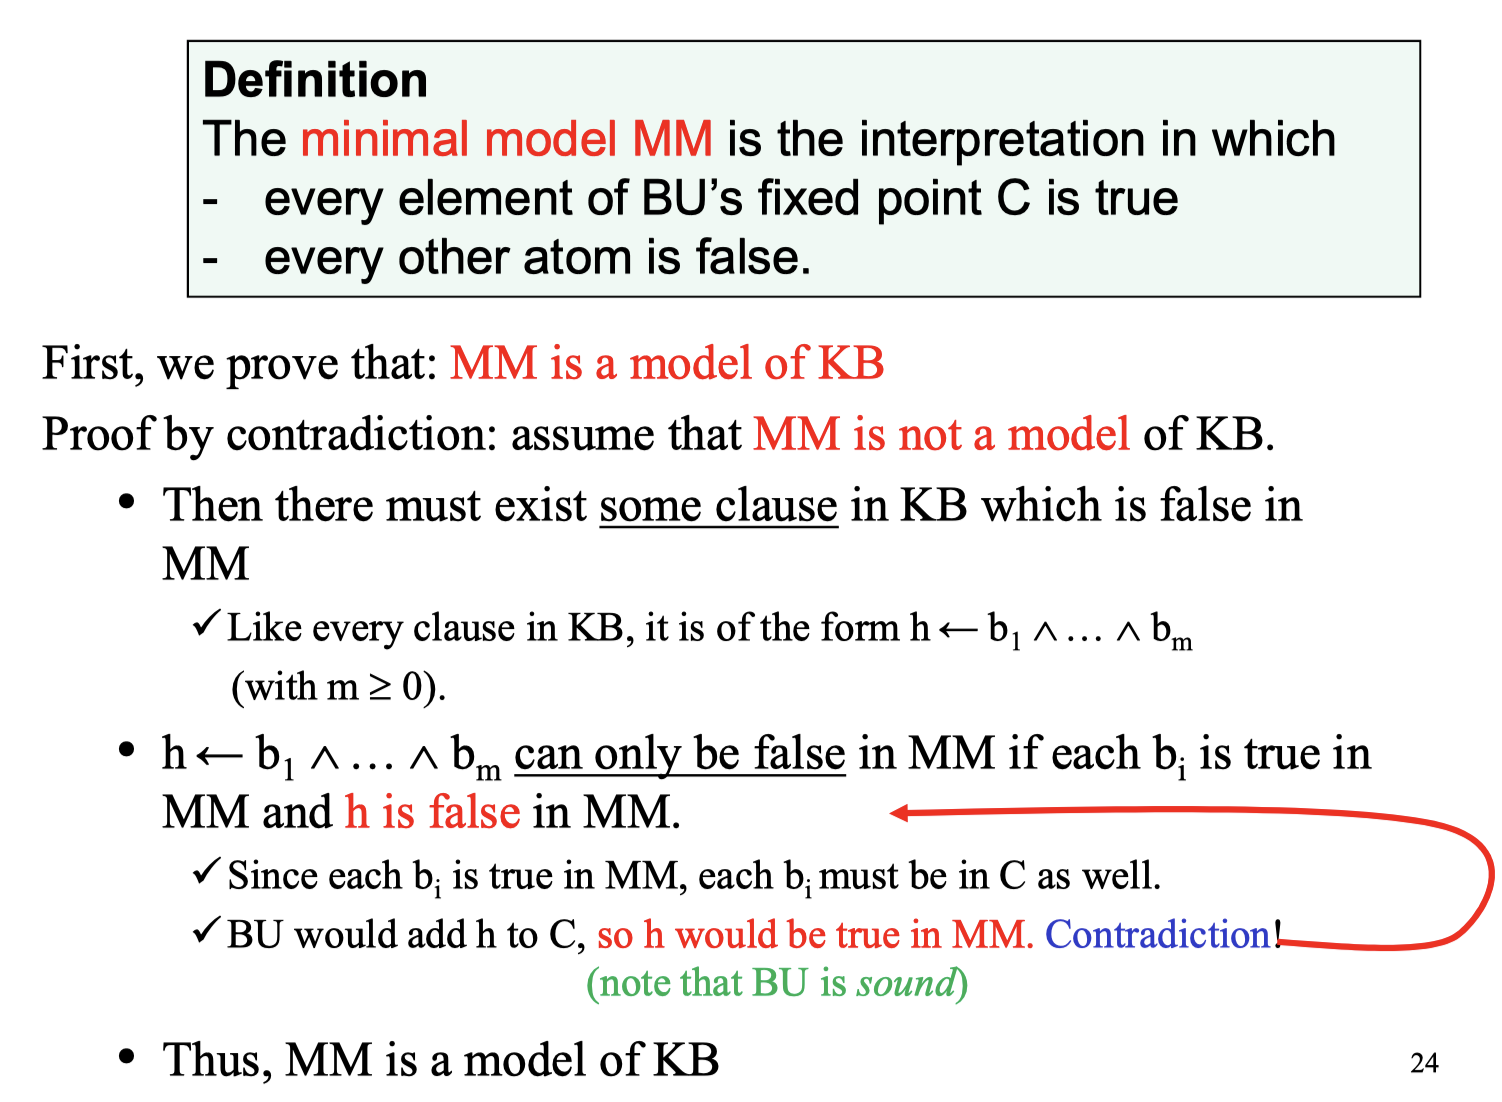
\includegraphics[scale=0.45]{completeness_of_bu}
\end{itemize}

\subsection{Top-Down Proof Procedure}

\begin{itemize}
    \item Proof procedure:
    \begin{algorithmic}
        \State{$ac := yes \leftarrow \text{body}$ (body is $q_1 \wedge \ldots \wedge q_k$)}
        \Repeat
            \State{Select $q_i \in \text{body}$}
            \State{Choose clause $c_i \in KB$, $c_i$ is $q_i \leftarrow b_c$}
            \State{Replace $q_i$ in body by $b_c$}
        \Until{$ac$ is an answer (fail if no clause with $q_i$ as head)}
    \end{algorithmic}
    \item
    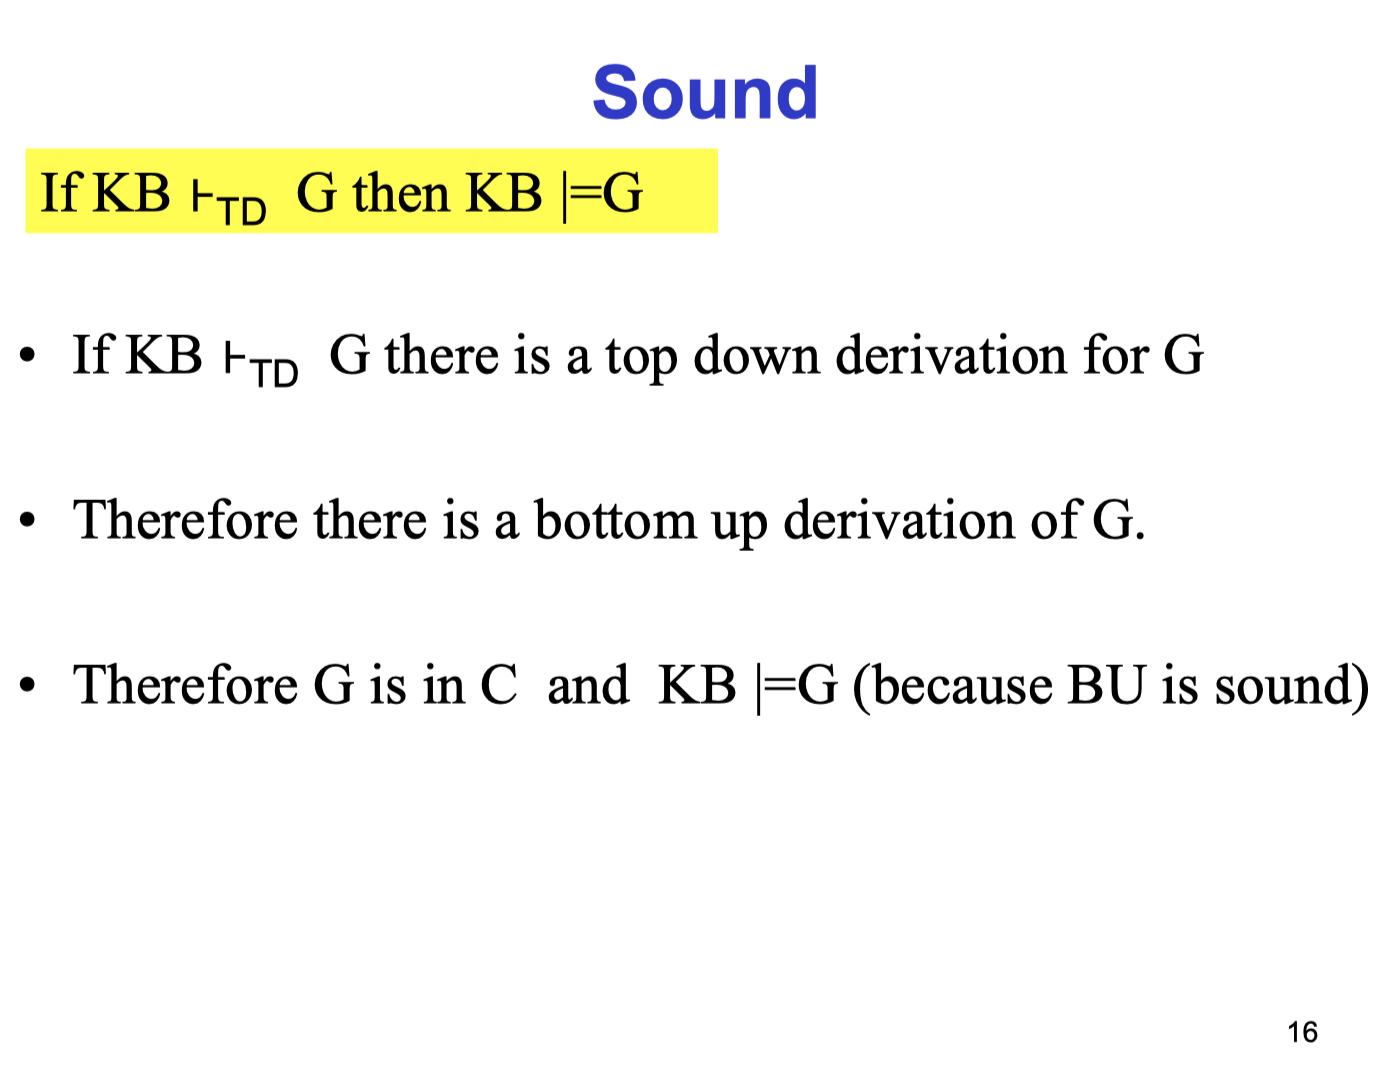
\includegraphics[scale=0.45]{soundness_of_td}
    \item
    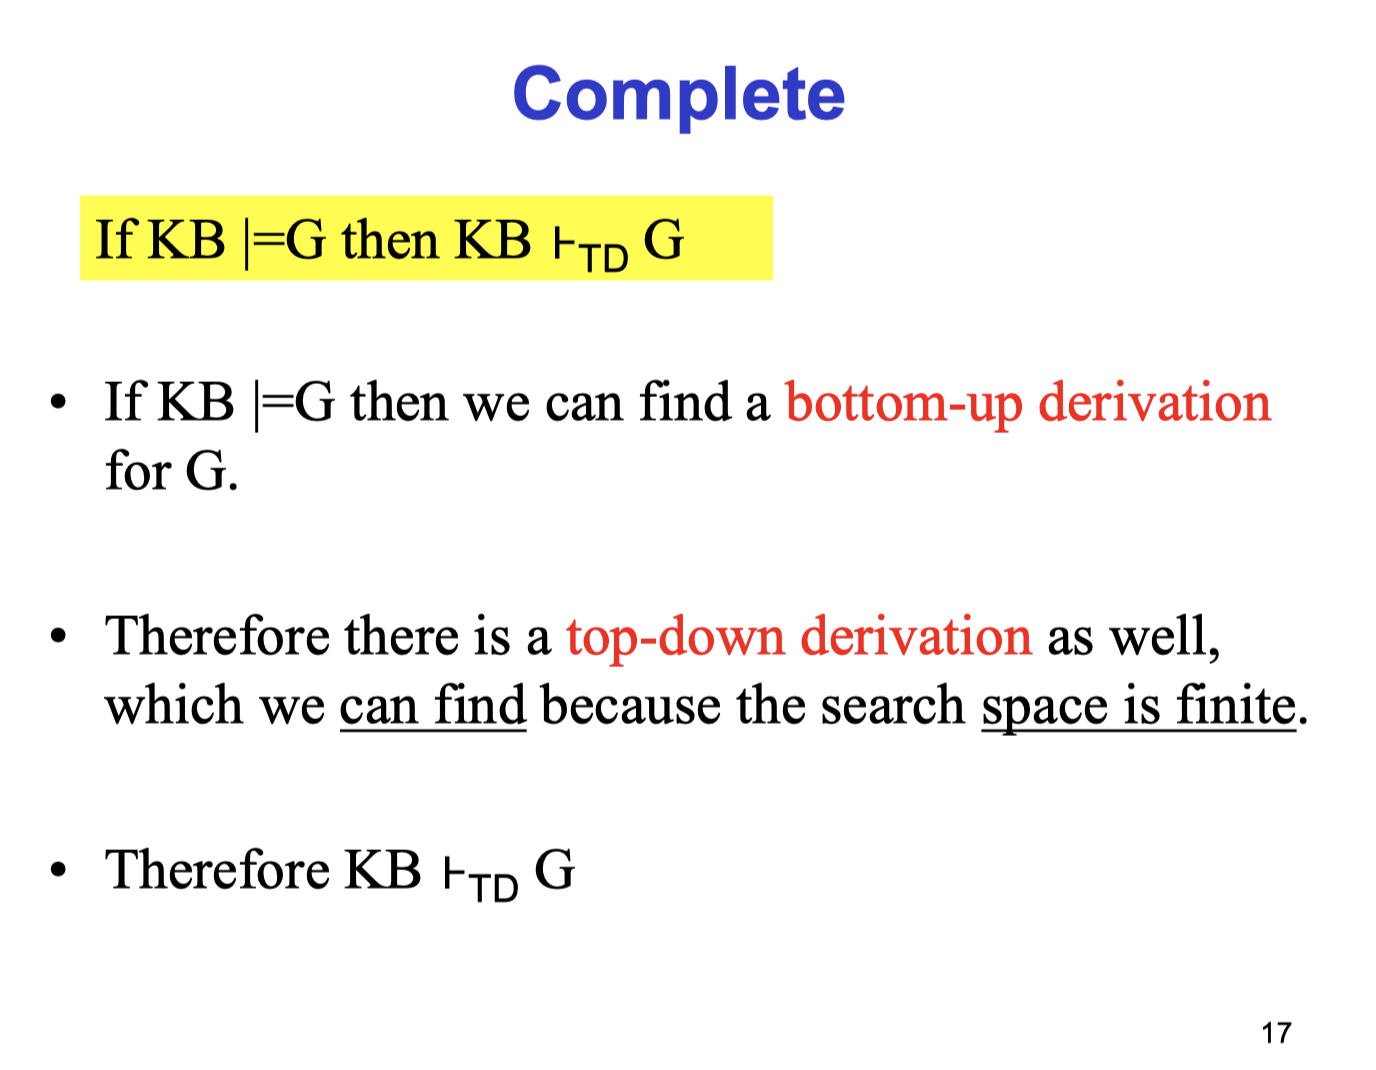
\includegraphics[scale=0.45]{completeness_of_td}
\end{itemize}

\subsection{Top-Down as Search}

\begin{itemize}
    \item query stated as an answer clause $\Rightarrow$ an answer
    \item \textbf{State}: answer clause of the form $\text{yes} \leftarrow a_1 \wedge \ldots \wedge a_k$
    \item Successor function: state resulting from submitting first atom $a_1$ with $b_1 \wedge \ldots \wedge b_m$ if there is a clause $a_1 \leftarrow b_1 \wedge \ldots \wedge b_m$
    \item \textbf{Goal test}: is the answer clause empty (i.e. $\text{yes} \leftarrow$)?
    \item \textbf{Solution}: the proof, i.e. sequence of SLD solutions
    \item \textbf{Heuristic function}: ???
\end{itemize}

\subsection{Datalog}

\begin{itemize}
    \item Datalog vs. PDCL

    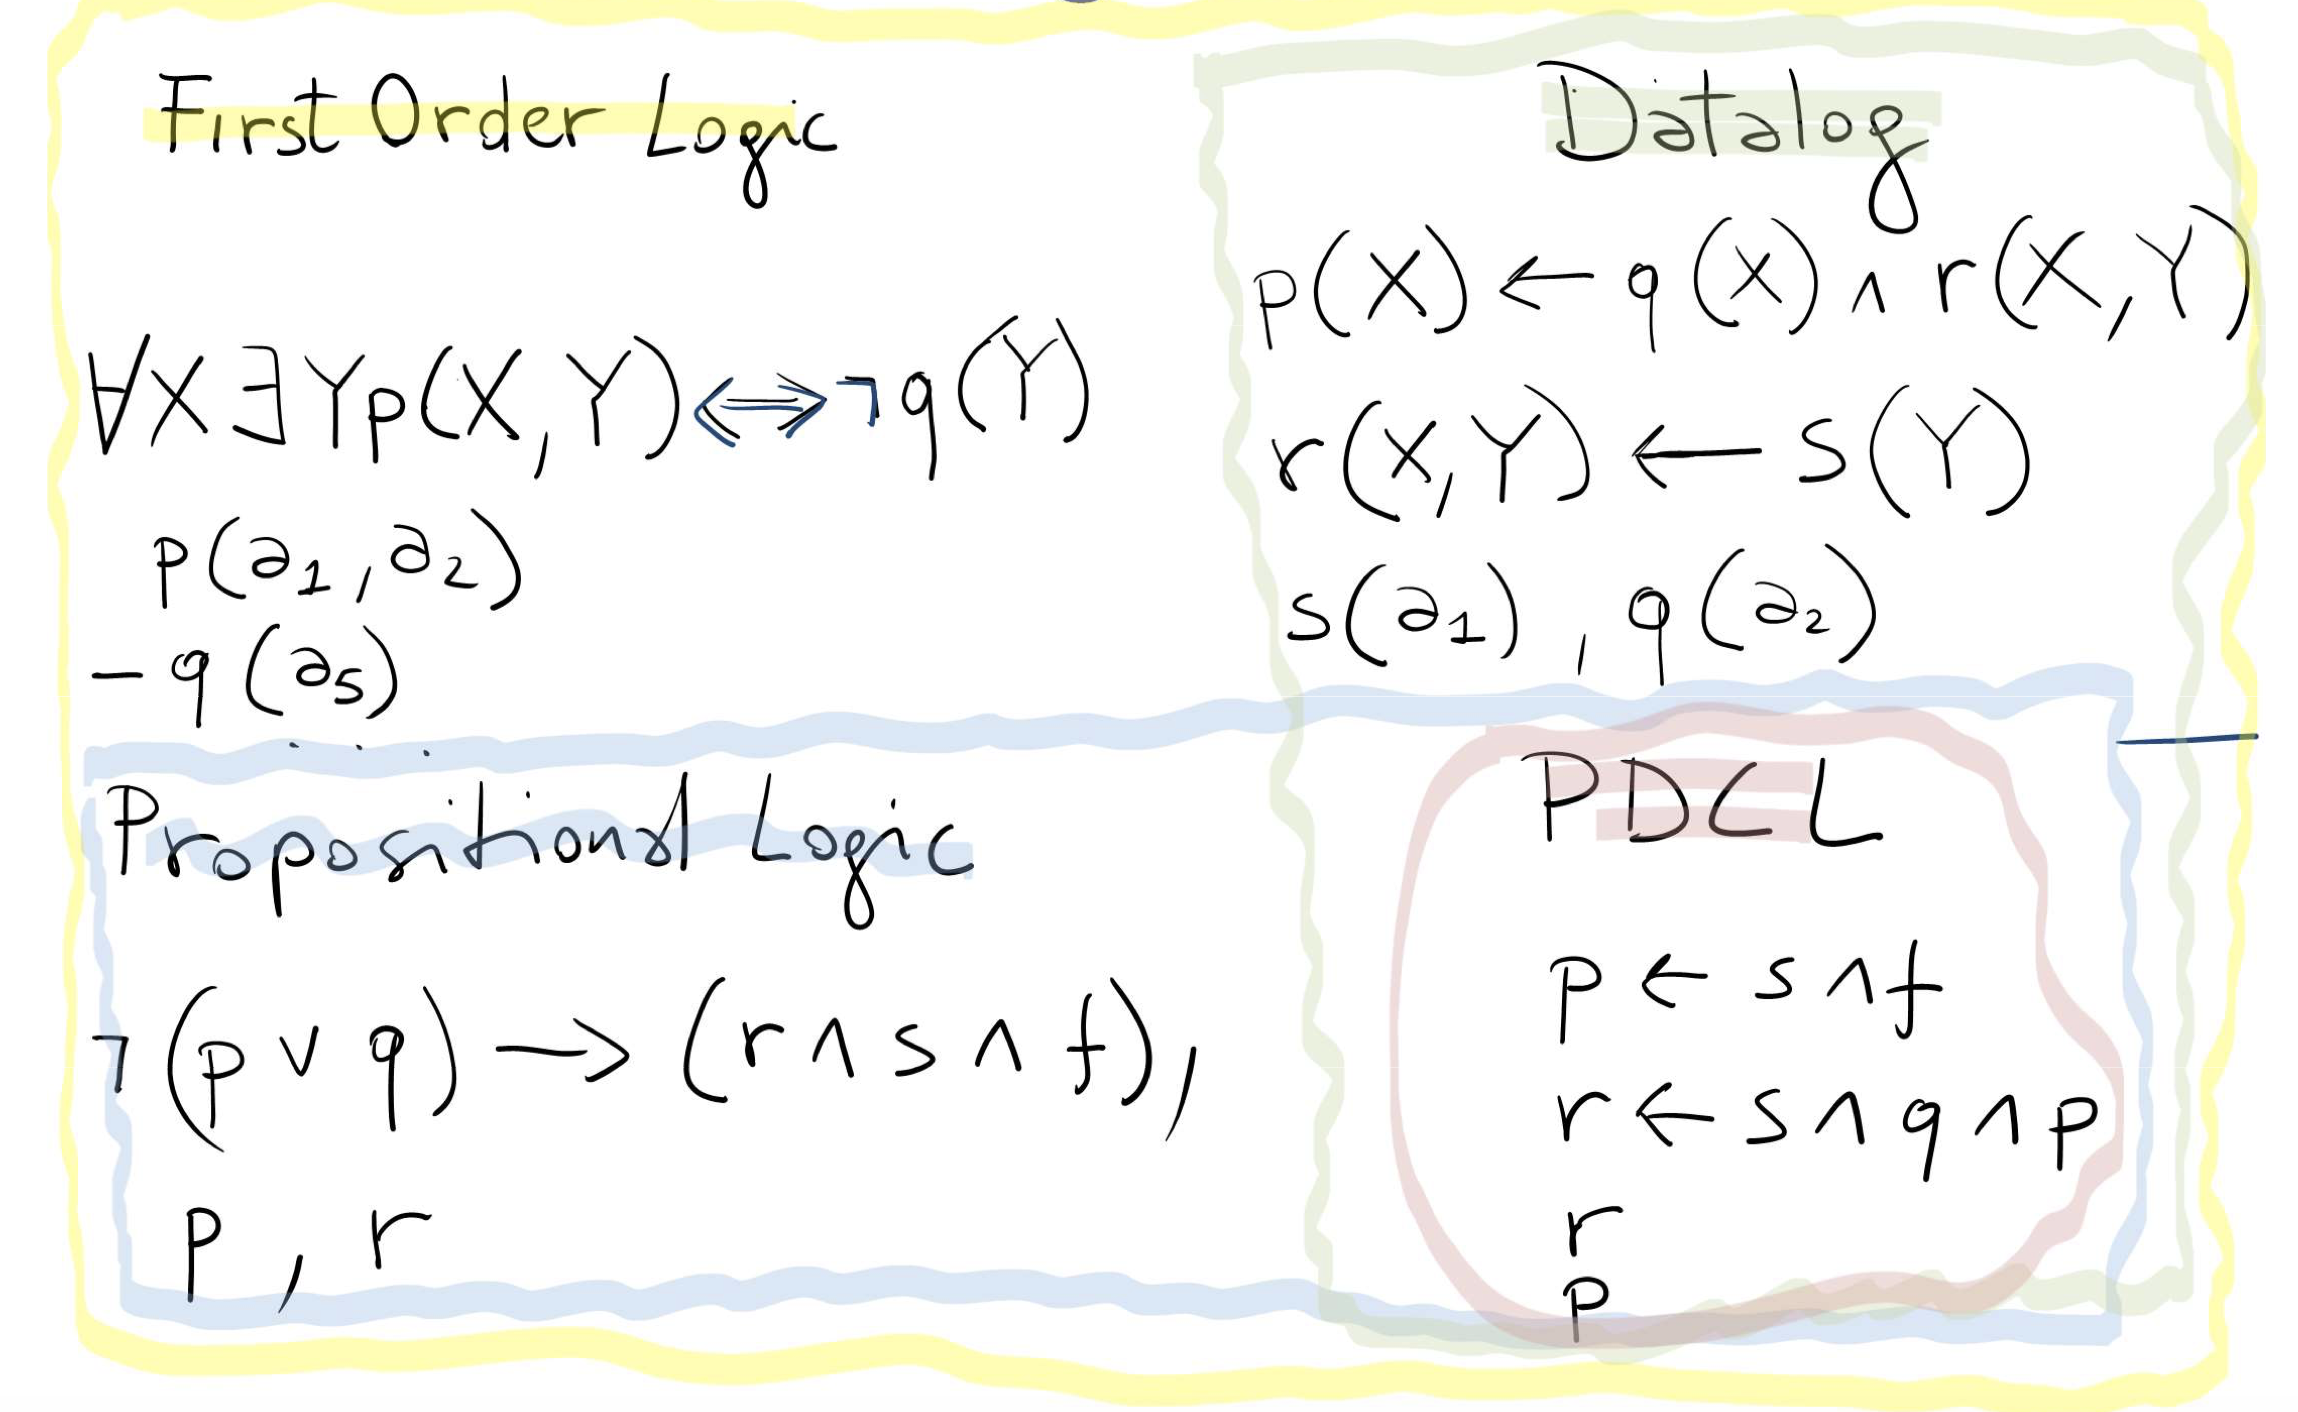
\includegraphics[scale=0.3]{datalog_vs_pdcl}
    \item Syntax
        \begin{itemize}
            \item \textbf{Variable}: symbol starting with an upper-case letter.
            \item \textbf{Constant}: symbol starting with a lower-case letter/a sequence of digits.
            \item \textbf{Term}: variable/constant.
            \item \textbf{Predicate symbol}: symbol starting with a lower-case letter.
            \item \textbf{Atom}: symbol of the form $p$/$p(t_1 \ldots t_n$ where $p$ is a predicate symbol and $t_i$ are terms.
            \item \textbf{Definite clause}: atom/of the form: $h$ and $b_i$ are atoms (``$h$ if $b$'')
            \item \textbf{KB} = set of definite clauses
        \end{itemize}
    \item Top-Down Proof Procedure (Lecture 21 Slides 9 - 11)
\end{itemize}

\section{Uncertainty: Probability Theory}

\subsection{Intro to Reasoning Under Uncertainty}

\begin{itemize}
    \item Two types of uncertainty:
        \begin{itemize}
            \item \textbf{Sensing uncertainty}: The agent cannot fully observe a state of interest.
            \item \textbf{Effect uncertainty}: The agent cannot be certain about the effects of its actions.
        \end{itemize}
    \item Belief in a proposition $f$ can be measured in terms of a number between 0 and 1.
\end{itemize}

\subsection{Intro to Probability}

\begin{itemize}
    \item \textbf{Probability theory}: system of logical axioms and formal operations for sound reasoning under uncertainty.
    \item \textbf{Basic element}: random variable $X$
        \begin{itemize}
            \item The agent can be uncertain about the value of $X$.
            \item Domain of $X$ = $dom(X)$
        \end{itemize}
    \item \textbf{Types of variables}: boolean, categorical,
    numeric.
    \item \textbf{Complex random variable}: a tuple of random variables $<X_1, \ldots, X_n>$ with domain $dom(X_1) \times dom(X_2) \times \ldots \times \ldots dom(X_n)$.
    \item \textbf{Assignment}: $X = x$ means $X$ has value $x$.
    \item \textbf{Proposition}: boolean formula made from assignment of values to variables.
    \item \textbf{Possible world}: an assignment to each random variable (possible worlds are mutually exclusive and exhaustive).
        \begin{itemize}
            \item $w \vDash f$ means proposition $f$ is true in world $w$.
            \item A probability measure $\mu(w)$ over possible worlds $w$ is a non-negative number such that $\mu(w)$ sums to 1 over all possible worlds $w$.
            \item $P(f) = \sum_{w \vDash f} \mu(w)$
        \end{itemize}
    \item \textbf{Probability distributions P}: on a random variable $X$ is a function $dom(X) \rightarrow [0, 1]$ such that $x \rightarrow P(X = x)$.
\end{itemize}

\subsection{Marginalization}

\begin{itemize}
    \item \textbf{Joint probability distribution (JPD)}: a probability distribution over the joint random variable $<X_1, \ldots, X_n>$.
        \begin{itemize}
            \item n-dimensional table of the corresponding possible worlds
                \begin{itemize}
                    \item row = assignment + probability
                    \item sum of probabilities = 1;
                \end{itemize}
        \end{itemize}
    \item \textbf{Marginalization}:
        \begin{equation*}
            P(\textcolor{blue}{X = x, Y = y, \ldots}) = \sum_{\textcolor{red}{z_1 \in dom(Z_1), \ldots, z_n \in dom(Z_n)}} P(\textcolor{blue}{X = x, Y = y, \ldots}, \textcolor{red}{Z_1 = z_1, \ldots, Z_n = Z_n})
        \end{equation*}
\end{itemize}

\subsection{Conditioning}

\begin{itemize}
    \item \textbf{Conditioning}: revise beliefs based on new observations
        \begin{itemize}
            \item Build on a probabilistic model (JPD).
                \begin{itemize}
                    \item \textbf{Prior probability distribution}: all background info ($P(h)$ = prior probability for hypothesis $h$).
                \end{itemize}
            \item Observe new information about the world.
                \begin{itemize}
                    \item \textbf{Evidence ($e$)}: info received subsequently.
                \end{itemize}
            \item Integrate the two sources of info.
                \begin{itemize}
                    \item \textbf{Conditional probability $P(h|e)$} (also called \textbf{Posterior probability})
                \end{itemize}
        \end{itemize}
    \item \textbf{Conditional probability}
        \begin{equation*}
            P(h|e) = \frac{P(h \wedge e)}{P(e)}
        \end{equation*}
        \begin{itemize}
            \item $P(e)$ = sum of probability for all worlds in which $e$ is true.
            \item $P(h \wedge e)$ = sum of probability for all worlds in which both $h$ and $e$ are true.
        \end{itemize}
\end{itemize}

\subsection{Inference by Enumeration}

\begin{itemize}
    \item Given
        \begin{itemize}
            \item JPD on a set of variables $X$
            \item specific values $e$ for the evidence variables $E$ (a subset of $X$)
        \end{itemize}
    \item Compute
        \begin{itemize}
            \item posterior joint distribution of query variables $Y$ (a subset of $X$)
        \end{itemize}
    \item Steps:
        \begin{enumerate}
            \item Condition to get distribution $P(X|e)$
            \item Marginalize to get distribution $P(Y|e)$
        \end{enumerate}
    \item Problems of inference by enumeration
        \begin{itemize}
            \item $n$ = number of variables, $d$ = size of the largest domain
            \item Space complexity: $O(d^n)$ possible worlds
            \item Time complexity: $O(d^n)$ sum over all entries in JPD
        \end{itemize}
\end{itemize}

\subsection{Bayes Rules}

\begin{align*}
    P(h|e) = \frac{P(h \wedge e)}{P(e)} \qquad &\text{and} \qquad P(e|h) = \frac{P(e \wedge h)}{P(h)} \\
    P(h \wedge e) &= P(h|e) \times P(e) \\
    P(e \wedge h) &= P(e|h) \times P(h) \\
    P(h \wedge e) &= P(e \wedge h) \\
    \Rightarrow P(h|e) &= \frac{P(e|h)P(h)}{P(e)}
\end{align*}

\subsection{Product Rule}

\begin{align*}
    P(f_2|f_1) &= \frac{P(f_2 \wedge f_1)}{P(f_2)} \\
    \Rightarrow P(f_2 \wedge f_1) &=  P(f_2|f_1) \times P(f_1) \\
    \Rightarrow P(\textcolor{blue}{f_n \wedge \ldots \wedge f_{i + 1} \wedge \textcolor{red}{f_i \wedge \ldots \wedge f_1}}) &x= P(\textcolor{blue}{f_n \wedge \ldots \wedge f_{i + 1} | \textcolor{red}{f_i \wedge \ldots \wedge f_1}}) \times P(\textcolor{red}{f_i \wedge \ldots \wedge f_1}) \tag{in general}
\end{align*}

\subsection{Chain Rule}

\begin{align*}
    P(\textcolor{blue}{f_2} \wedge \textcolor{red}{f_1}) &= P(\textcolor{blue}{f_2}|\textcolor{red}{f_1}) \times P(\textcolor{red}{f_1}) \\
    P(\textcolor{blue}{f_n} \wedge \textcolor{red}{f_{n-1} \wedge \ldots \wedge f_1}) &= P(\textcolor{blue}{f_n} | \textcolor{red}{f_{n-1} \wedge \ldots \wedge f_1}) \times P(\textcolor{red}{f_{n-1} \wedge \ldots \wedge f_1}) \tag{in general} \\
    &= P(\textcolor{blue}{f_n} | \textcolor{red}{f_{n-1} \wedge \ldots \wedge f_1}) \times P(\textcolor{red}{f_{n-1}} | \textcolor{green}{f_{n-2} \wedge \ldots \wedge f_1}) \times P(\textcolor{green}{f_{n-2} \wedge \ldots \wedge f_1}) \\
    &= \ldots \\
    P(f_1 \wedge \ldots \wedge f_n) &= \prod\limits_{i = 1}^{n} P(f_i|f_{i - 1} \wedge \ldots \wedge f_1)
\end{align*}

\subsection{Marginal Independence}

\begin{itemize}
    \item \textbf{Marginal independence}: Random variable $X$ is (marginally independent) of random variable $Y$ ($X \bigCI Y$), if for all $x_i \in dom(X), y_i \in dom(Y)$ and $y_k \in dom(Y)$, the following equation holds:
    \begin{align*}
        P(X = x_i|Y = y_i) &=  P(X = x_i|Y = y_k) \\
        &= P(X = x_i)
    \end{align*}
\end{itemize}

\subsection{Conditional Independence}

\begin{itemize}
    \item \textbf{Conditional independence}: Random variable $X$ is conditionally independent of random variable $Y$ given random variable $Z$ if, for all $x_i \in dom(X), y_i \in dom(Y), y_k \in dom(Y)$ and $z_m \in dom(Z)$ the following equation holds:
    \begin{align*}
        P(X = x_i|Y = y_i, Z = z_m) &= P(X = x_i|Y = y_k, Z = z_m) \\
        &= P(X = x_i|Z = z_m)
    \end{align*}
\end{itemize}

\section{Appendix}

\subsection{Learning Goals}

\subsubsection*{Search}

\begin{itemize}
    \item Identify real world examples that make use of deterministic, goal-driven planning agents.
    \item Assess the size of the search space of a given search problem.
    \item Trace through/implement a generic search algorithm.
    \item Determine basic properties of search algorithms: completeness, optimality, time and space complexity of search algorithms.
    \item Select the most appropriate search algorithms for specific problems:
        \begin{itemize}
            \item BFS vs. DFS vs. IDS
            \item LCFS vs. BestFS
            \item A* vs B\&B vs. IDA* vs MBA*
        \end{itemize}
    \item Define/read/write/trace/debug different search algorithms
        \begin{itemize}
            \item With/without cost
            \item Informed/uninformed
        \end{itemize}
    \item Construct admissible heuristics for a given problem.
    \item Verify Heuristic Dominance.
    \item Combine admissible heuristics.
    \item Formally prove A* optimality.
    \item Justify and describe methods for pruning cycles and repeated states (multiple paths).
\end{itemize}

\subsubsection*{CSP}

\begin{itemize}
    \item Define possible worlds in terms of variables and their domains.
    \item Compute number of possible worlds on real examples.
    \item Specify constraints to represent real world problems differentiating between:
        \begin{itemize}
            \item Unary and k-ary constraints
            \item List vs. function format
        \end{itemize}
    \item Verify whether a possible world satisfies a set of constraints (i.e. whether it is a model, a solution)
    \item Implement the Generate-and-Test Algorithm. Explain disadvantages.
    \item Solve a CSP by search (specify neighbours, states, start state, goal state). Compare strategies for CSP search. Implement pruning for DFS search in CSP.
    \item Build a constraint network for a set of constraints.
    \item Verify whether a network is arc consistent.
    \item Make an arc arc-consistent.
    \item Define/read/write/trace/debug the arc consistency algorithm. Compute its complexity and assess its possible outcomes.
    \item Define/read/write/trace/debug domain splitting and its integration with arc consistency.
    \item Local search for a CSP
        \begin{itemize}
            \item different ways to generate neighbours
            \item scoring functions to solve a CSP by local search
                \begin{itemize}
                    \item through either greedy descent/hill climbing
                \end{itemize}
        \end{itemize}
    \item Implement SLS with
        \begin{itemize}
            \item random steps (1-step, 2-step versions)
            \item random descent
        \end{itemize}
    \item Compare SLS algorithms with runtime distributions.
    \item Implement the simulated annealing algorithm.
    \item Implement a Taboo list.
    \item Explain pros and cons of different SLS algorithms.
\end{itemize}

\subsubsection*{Planning}

\begin{itemize}
    \item Represent a planning problem with the STRIPS representation.
    \item Explain the STRIPS assumption.
    \item Solve a planning problem by search (forward planning). Specify states, successor function, goal test and solution.
    \item Construct and justify a heuristic function for forward planning.
    \item Translate a planning problem represented in STRIPS into a corresponding CSP problem (and vice versa).
    \item Solve a planning problem with CSP by expanding the horizon.
\end{itemize}

\subsubsection*{Logic}

\begin{itemize}
    \item PDCL syntax \& semantics
        \begin{itemize}
            \item Verify whether a logical statement belongs to the language of propositional definite clauses.
            \item Verify whether an interpretation is a model of a PDCL KB.
            \item Verify when a conjunction of atoms is a logical consequence of a KB.
        \end{itemize}
    \item Bottom-up proof procedure
        \begin{itemize}
            \item Define/read/write/trace/debug the Bottom Up (BU) proof procedure.
            \item Prove that the BU proof procedure is sound and complete.
        \end{itemize}
    \item Top-down proof procedure
        \begin{itemize}
            \item Define/read/write/trace/debug the Top-down (SLD) proof procedure.
            \item Prove that the TD proof procedure is sound and complete.
        \end{itemize}
    \item Datalog
        \begin{itemize}
            \item Represent simple domains in Datalog.
            \item Apply the Top-down proof procedure in Datalog.
        \end{itemize}
\end{itemize}

\subsubsection*{Uncertainty: Probability Theory}

\begin{itemize}
    \item Define and give examples of random variables, their domains and probability distributions.
    \item Calculate the probability of a proposition f given µ(w) for the set of possible worlds.
    \item Given a JPD:
        \begin{itemize}
            \item Marginalize over specific variables.
            \item Compute distributions over any subset of the variables.
        \end{itemize}
    \item Apply the formula to compute conditional probability $P(h|e)$.
    \item Use inference by enumeration:
        \begin{itemize}
            \item to compute joint posterior probability distributions over any subset of variables given evidence.
        \end{itemize}
    \item Derive and use Bayes Rule.
    \item Derive the Chain Rule.
    \item Define and use marginal independence.
    \item Define and use conditional independence.
\end{itemize}

\subsubsection*{Uncertainty: Belief Networks}

\begin{itemize}
    \item Build a Bayesian Network for a given domain.
    \item Identify the necessary CPTs.
    \item Compare different network structures.
    \item Understand dependencies and independencies.
    \item Variable elimination
        \begin{itemize}
            \item Understating factors and their operations.
            \item Carry out variable elimination by using factors and the related operations.
            \item Use techniques to simplify variable elimination.
        \end{itemize}
\end{itemize}

\end{document}
